\documentclass[tikz,border=10pt]{standalone}
\usetikzlibrary{calc}

\begin{document}
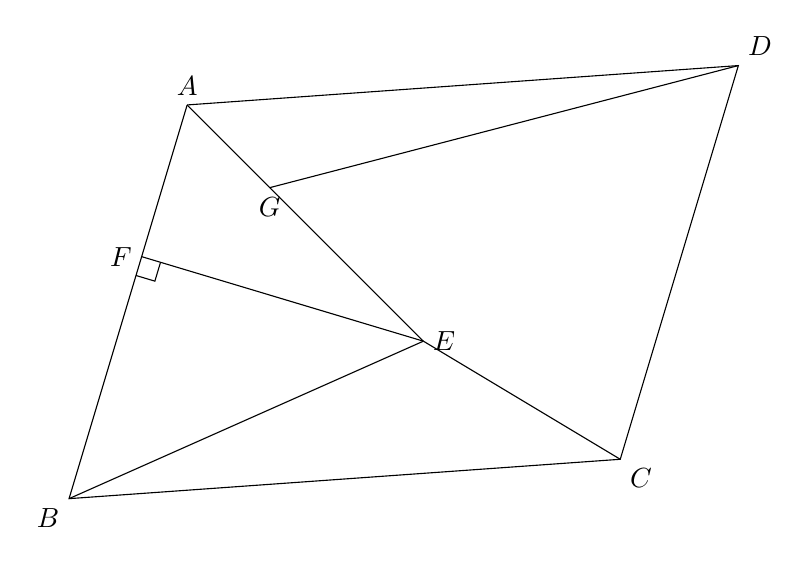
\begin{tikzpicture}
    % Define coordinates
    \coordinate (B) at (1,1);
    \coordinate (C) at (8,1.5);
    \coordinate (A) at (2.5,6);
    \coordinate (D) at (9.5,6.5);
    
    % Point E
    \coordinate (E) at (5.5,3);
    
    % Point F: Projection of E onto AB
    \coordinate (F) at ($(A)!(E)!(B)$);
    
    % Point G: On AE, closer to A
    \coordinate (G) at ($(A)!0.35!(E)$);
    
    % Draw Quadrilateral ABCD
    \draw (A) -- (B) -- (C) -- (D) -- (A);
    
    % Draw internal segments
    \draw (A) -- (E); 
    \draw (D) -- (G); 
    \draw (B) -- (E); 
    \draw (C) -- (E); 
    \draw (E) -- (F); 
    
    % Right angle mark at F
    \coordinate (F1) at ($(F)!0.25cm!(B)$);
    \coordinate (F2) at ($(F)!0.25cm!(E)$);
    \coordinate (F3) at ($(F1) + (F2) - (F)$);
    \draw (F1) -- (F3) -- (F2);
    
    % Labels
    \node[above] at (A) {$A$};
    \node[below left] at (B) {$B$};
    \node[below right] at (C) {$C$};
    \node[above right] at (D) {$D$};
    \node[right] at (E) {$E$};
    \node[left] at (F) {$F$};
    \node[below] at (G) {$G$};
\end{tikzpicture}
\end{document}
